\documentclass[../interim.tex]{subfiles}



\begin{document}

\section{Background}

This section introduces some technical background which will likely be required as part of the project. It includes an introduction to neural networks and CNNs, a comparison of some existing object tracking and object detection algorithms and a discussion on knowledge representation and reasoning and symbolic rule learning.

\subsection{Deep Learning}

Deep neural networks (DNNs) have emerged as a very successful algorithm for machine learning; deep learning has been used to beat records in tasks such as image recognition, speech recognition and language translation\cite{deep-learning-intro}. Many different architectures have been proposed to solve various tasks, these architectures include convolutional neural networks (CNNs), which are designed to process data that come in the form of multiple arrays\cite{deep-learning-intro}, and recurrent neural networks (RNNs), which are designed to process sequences of arbitrary length\cite{def:rnn}. The following section gives a brief introduction to CNNs and describes some of their use cases.

\subsubsection{Convolutional Neural Networks}

CNNs contain three types of layers: convolution, pooling and fully connected. Units (artificial neurons) in a convolution layer are organised into feature maps. The inputs to each unit in a feature map come from the outputs of the units in a small region of the previous layer, the output of the unit is then calculated by passing the weighted sum of its inputs through an activation function such as ReLU. The set of weights, also known as a filter or kernel, is the part of the layer which is learned through backpropagation. Every unit in a feature map has the same kernel. Each feature map in a layer has its own kernel. Pooling layers reduce the size of the input by merging multiple units into one. A typical pooling operation is max-pooling, which computes the maximum of a local patch of units. Finally, in fully-connected layers (which are typically placed at the output of the CNN) every unit in a layer is connected to every unit in the previous layer. An example CNN architecture is shown in Figure~\ref{fig:example-cnn}.

\begin{figure}
  \centering
  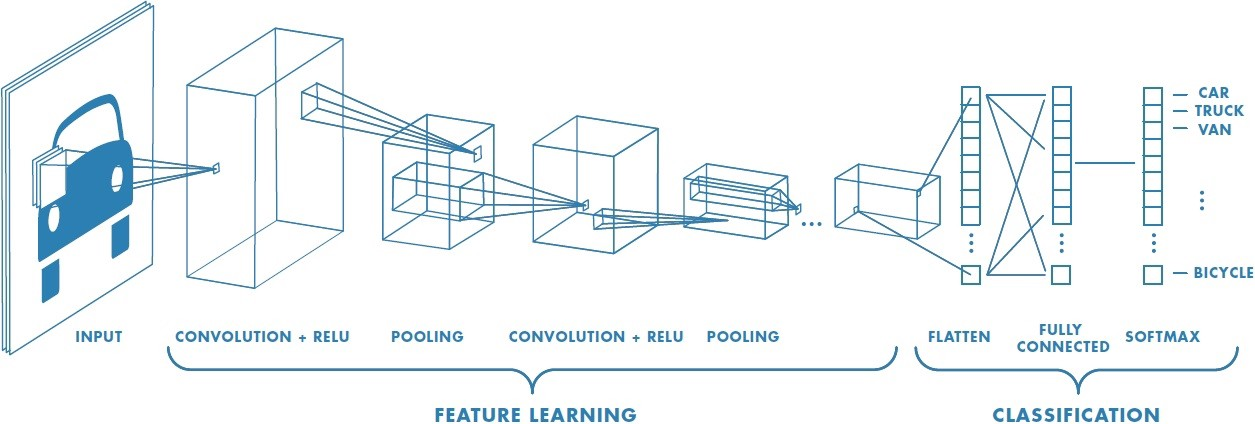
\includegraphics[width=0.8\textwidth]{cnn-example.jpg}
  \label{fig:example-cnn}
  \caption{An example of a CNN architecture. The input image is passed through a series of convolution and pooling layers before begin flattened into a one-dimensional layer and passed through one final fully connected layer. The softmax classification function is then applied at the output.}
\end{figure}

CNNs have proven to be adept at a number of tasks involving images, including image classification\cite{cnn-uses:classification} and object detection\cite{cnn-uses:yolo-v3}\cite{cnn-uses:faster-r-cnn}. We explore these further in Section~\ref{section:image-proc}.


\subsection{Image Processing}
\label{section:image-proc}


\end{document}
